\documentclass[a4paper]{article}

\usepackage[table]{xcolor}%this has to be the first!!!!!!
\usepackage{fullpage} % Package to use full page
%\usepackage{parskip} % Package to tweak paragraph skipping
\usepackage{tikz} % Package for drawing
\usetikzlibrary{shapes,arrows,matrix,positioning}
\usepackage{amsmath}
\usepackage{indentfirst}
\usepackage{hyperref}
\usepackage{subcaption}
\usepackage{graphics}
\usepackage{graphicx}
\usepackage{minted}
\usepackage{multicol}
\usepackage{mathrsfs}
%color define
\definecolor{codebg}{RGB}{230,255,253}
\definecolor{function}{RGB}{210,0,26}
\definecolor{para}{RGB}{255,137,137}
\definecolor{output}{RGB}{238,224,201}
\setminted[cpp]{mathescape=true,breaklines,bgcolor=codebg,linenos}

\tikzset{
  block/.style = {rectangle, draw, fill=output, text width=6cm, text centered, rounded corners, minimum height=4em},
  line/.style = {draw, -latex'},
}

%function newcommand
\newcommand{\func}[1]{\textbf{\textcolor{function}{#1}}}
\newcommand{\para}[1]{\textbf{\emph{\textcolor{para}{#1}}}}

%other examples for icon in text
%WARNING: the number is not allowed in newcommand name
\newcommand{\testA}{\tikz \fill[brown] (2pt,2pt) rectangle (8pt,8pt);}
\newcommand{\testB}{\tikz \fill[black] (3pt,3pt) circle (3pt);}

\usepackage{biblatex}
\addbibresource{bibliography.bib}
\title{readme}
\author{Haochen(Langford) Huang}
\date{\today}

\makeatletter%title setting
\def\@maketitle{%
  \newpage
  \null
  \vskip 2em%
  \begin{center}%
  \let \footnote \thanks
    {\LARGE \@title \par}%
    \vskip 1.5em%
    {\Large
      \lineskip .5em%
      \begin{tabular}[t]{c}%
        \@author
      \end{tabular}\par}%
    \vskip 1em%
    {\large \@date\par}%
    \vskip 1em%
    {\large version:2.0}%
  \end{center}%
  \par
  \vskip 1.5em}
\makeatother

\begin{document}

\maketitle

\section{Readme}
Normally, a documentation would consist of two major parts: Introduction \& Backround and Function. The first part will introduce the purpose of the corresponding program and the governing equations it solved and other thing developers and users should be aware of \emph{e.g.} in which method the program solve the overall problem. Pragmatic program will be explored line by line in the second part. It first contains a table to clearify all the parameters and their physical representatives as shown in Table.\ref{tab:test}. 
\begin{table}[h]
  \centering
  \begin{tabular}{|c|c|c|c|c|}
    \hline
    Name & Data type & Status & Option & Representation (before/after)\\[0.5ex]
    \hline\hline
    \rowcolor{output} \para{a} & scalar* & update & complusory & $\delta \mathbf{u}^{*,k}/\delta \mathbf{u}^{*,k+1}$\\
    \hline
    \para{b} & scalar* & unchange & complusory & $RES$\\
    \hline
    \para{dt} & double & unchange & complusory & $\Delta t$\\
    \hline
    \para{l} & int & unchange & complusory &  mesh level \\
    \hline
    \para{data} & struct Vsicosity & unchange & complusory & $\mu^ {n+\frac{1}{2}}, \rho^{n+\frac{1}{2}}, \Delta t$ \\
    \hline
  \end{tabular}
  \caption{Referenc table of parameters.}
  \label{tab:test}
\end{table}
The highlighted row in the table indicates such paramter is either the output or has been updated. Second subsection always concerns with detals and specific technique the function employed. Finally the third part is the workflow of the program.\par
Throughout documentation font \para{para} represents exact name of parameters and \func{function} represents exact name of the function.

Tikz inside text example: $\testA$.

\section{Program Workflow Example}
\begin{multicols}{2}
  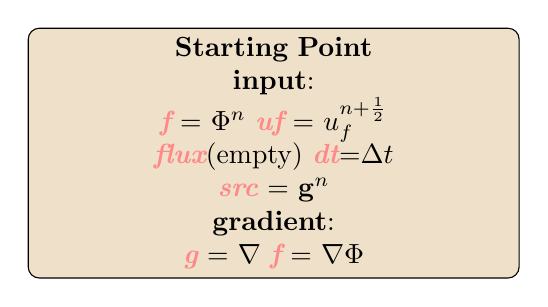
\begin{tikzpicture}
    \node [block](init){
        \textbf{Starting Point}\\
        \textbf{input}: \\
        \para{f} = $\Phi^n$ \para{uf} = $u_f^{n+ \frac{1}{2}}$\\ \para{flux}(empty) \para{dt}=$\Delta t$\\ \para{src} = $ \mathbf{g}^n$\\
        \textbf{gradient}:\\
        \para{g} = $\nabla$ \para{f} = $\nabla \Phi$
      };
  \end{tikzpicture}
 \columnbreak
 \begin{minted}{cpp}
void tracer_fluxes (scalar f,
		    face vector uf,
		    face vector flux,
		    double dt,
		    (const) scalar src)
{
  vector g[];
  gradients ({f}, {g});
 \end{minted}
 
\end{multicols}

\begin{center}
  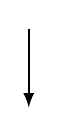
\begin{tikzpicture}
    \draw[-latex,thick](0,0) -- (0,-1); 
  \end{tikzpicture}
\end{center}

\printbibliography
\end{document}
